\chapter{Μεθοδολογία}

\section{Εισαγωγή στη Μεθοδολογία}

Το παρόν κεφάλαιο παρουσιάζει τον πειραματικό σχεδιασμό που αναπτύχθηκε για τη διερεύνηση τριών θεμελιωδών ερευνητικών υποθέσεων σχετικά με την εφαρμογή ασαφών μεθόδων στην ανάλυση δεδομένων αισθητήρων.
Η μεθοδολογία που ακολουθείται στοχεύει στη συστηματική αξιολόγηση της προτεινόμενης προσέγγισης μέσω ελεγχόμενων πειραμάτων, στατιστικής επικύρωσης και συγκριτικής ανάλυσης με υπάρχουσες τεχνικές.
Ο σχεδιασμός εστιάζει στην αναπαραγωγιμότητα των αποτελεσμάτων και την εξασφάλιση της επιστημονικής εγκυρότητας μέσω αυστηρών πρωτοκόλλων αξιολόγησης.

Η συνολική προσέγγιση ξεκινά από την επεξεργασία ακατέργαστων σημάτων πολλαπλών αισθητήρων και καταλήγει στον υπολογισμό ασαφών μετρικών ομοιότητας μεταξύ χρονικών παραθύρων δραστηριοτήτων.
Η μετάβαση από τα αριθμητικά δεδομένα αισθητήρων σε ασαφείς συναρτήσεις συμμετοχής επιτυγχάνεται κυρίως μέσω του αλγορίθμου \en{Normalized Difference Gaussian Streaming (NDG-S)}\cite{Truong2012}, ο οποίος αποδεικνύεται υπολογιστικά αποδοτικός, ενώ διατηρεί παράλληλα την ακρίβεια της αναπαράστασης.
Πέρα από την κατασκευή των ασαφών συναρτήσεων συμμετοχής, τα σήματα αισθητήρων υποβάλλονται σε προεπεξεργασία ώστε να εξαλειφθούν πιθανά περιβάλλοντα θορύβου, να κανονικοποιηθούν και να χωριστούν σε επικαλυπτόμενα χρονικά παράθυρα.

Η μεθοδολογία συνδέεται άμεσα με τα τρία βασικά ερευνητικά ερωτήματα που καθοδηγούν την έρευνα.
Το πρώτο ερευνητικό ερώτημα (ΕΕ1) εξετάζει την υπολογιστική αποδοτικότητα και ακρίβεια του αλγορίθμου \en{NDG-S} σε σύγκριση με την κλασική μέθοδο \en{Kernel Density Estimation (KDE)}, εστιάζοντας σε μετρικές απόδοσης όπως ο χρόνος εκτέλεσης και η κατανάλωση μνήμης.
Το δεύτερο ερώτημα (ΕΕ2) διερευνά την αποτελεσματικότητα ανάκτησης δραστηριοτήτων με βάση μετρικές ομοιότητας ασαφών συνόλων.
Το τρίτο ερώτημα (ΕΕ3) εξετάζει την ευστάθεια και γενικευσιμότητα των προτεινόμενων μετρικών μεταξύ ετερογενών συνόλων δεδομένων με διαφορετικά χαρακτηριστικά δειγματοληψίας και διατάξεις αισθητήρων.

Το κεφάλαιο δομείται σε διακριτές ενότητες που καλύπτουν όλες τις πτυχές του πειραματικού σχεδιασμού.
Αρχικά παρουσιάζεται το θεωρητικό πλαίσιο και οι βασικές αρχές που διέπουν τη μεθοδολογία, ακολουθούμενες από λεπτομερή περιγραφή των συνόλων δεδομένων και των διαδικασιών προεπεξεργασίας.
Στη συνέχεια αναλύονται οι τεχνικές λεπτομέρειες της δημιουργίας ασαφών συναρτήσεων συμμετοχής και η τεχνική σύγκρισης των ασαφών μετρικών ομοιότητας.
Το κεφάλαιο ολοκληρώνεται με την παρουσίαση του πλαισίου αξιολόγησης, των στατιστικών μεθόδων επικύρωσης και των μετρικών αξιολόγησης.
Η μετάβαση από τις θεωρητικές βάσεις στις τεχνικές υλοποίησης γίνεται σταδιακά, εξασφαλίζοντας την πλήρη κατανόηση κάθε συνιστώσας της μεθοδολογίας.

\section{Ερευνητικός Σχεδιασμός και Προσέγγιση}
Η παρούσα έρευνα υιοθετεί μια αυστηρά ποσοτική και υπολογιστική προσέγγιση για τη διερεύνηση
της αποτελεσματικότητας των ασαφών μετρικών ομοιότητας στην αναγνώριση ανθρώπινων
δραστηριοτήτων από δεδομένα αισθητήρων.
Η μεθοδολογία βασίζεται σε ελεγχόμενα πειράματα με επαναλαμβανόμενες μετρήσεις, στατιστική
επικύρωση αποτελεσμάτων και συστηματική σύγκριση εναλλακτικών προσεγγίσεων.
Κάθε πειραματική υπόθεση αξιολογείται μέσω αντικειμενικών μετρικών απόδοσης, εξασφαλίζοντας
την αναπαραγωγιμότητα και την επιστημονική εγκυρότητα των συμπερασμάτων.

Ο σχεδιασμός δίνει έμφαση στην εμπειρική επαλήθευση μέσω εκτεταμένων πειραμάτων σε δύο
καθιερωμένα σύνολα δεδομένων (\en{Opportunity} και \en{PAMAP2}).
Η επιλογή πολλαπλών συνόλων δεδομένων επιτρέπει τον έλεγχο της γενικευσιμότητας των
προτεινόμενων μεθόδων σε διαφορετικές συνθήκες δειγματοληψίας, τύπους αισθητήρων και
κατηγορίες δραστηριοτήτων, και θέτει τον ιδανικό στόχο για την διπλωματική εργασία.

Η εφαρμογή ασαφούς λογικής στην αναγνώριση ανθρώπινων δραστηριοτήτων προσφέρει σημαντικά
πλεονεκτήματα έναντι των παραδοσιακών προσεγγίσεων, ιδιαίτερα στη διαχείριση της εγγενούς
αβεβαιότητας και μεταβλητότητας των δεδομένων αισθητήρων.
Οι ανθρώπινες δραστηριότητες δεν εκτελούνται με απόλυτη ακρίβεια και επαναληψιμότητα, αλλά
παρουσιάζουν φυσικές διακυμάνσεις στην ταχύτητα, την ένταση και τον τρόπο εκτέλεσης μεταξύ
διαφορετικών ατόμων ή ακόμα και του ίδιου ατόμου σε διαφορετικές χρονικές στιγμές.
Η ασαφής λογική επιτρέπει τη μοντελοποίηση αυτής της στοχαστικότητας μέσω συναρτήσεων
συμμετοχής που αποδίδουν βαθμούς συμμετοχής αντί για δυαδικές κατηγοριοποιήσεις.

Επιπλέον, τα δεδομένα αισθητήρων χαρακτηρίζονται από θόρυβο, παρεμβολές και
περιστασιακές αστοχίες αισθητήρων που καθιστούν προβληματική την εφαρμογή αυστηρών κατωφλίων
και ντετερμινιστικών κανόνων.
Οι ασαφείς μετρικές ομοιότητας προσφέρουν ανθεκτικότητα σε τέτοιες διαταραχές, καθώς η
σύγκριση γίνεται σε επίπεδο κατανομών πιθανότητας και όχι σημειακών τιμών.
Η προτεινόμενη μέθοδος σύγκρισης ανά αισθητήρα ενισχύει περαιτέρω αυτή την ανθεκτικότητα,
διατηρώντας τα ιδιαίτερα χαρακτηριστικά κάθε αισθητήρα και αποφεύγοντας την απώλεια
πληροφορίας που συμβαίνει κατά τη συγχώνευση δεδομένων σε ενιαίες αναπαραστάσεις.

Η προτεινόμενη μεθοδολογία διαφοροποιείται ουσιαστικά από τις κλασικές προσεγγίσεις μηχανικής
μάθησης που κυριαρχούν στον τομέα της αναγνώρισης δραστηριοτήτων.
Οι παραδοσιακοί ταξινομητές όπως τα \en{Support Vector Machines (SVM)}, τα \en{Random
Forests} και τα νευρωνικά δίκτυα απαιτούν εκτεταμένη εξαγωγή χαρακτηριστικών (\en{feature
engineering}) και βασίζονται σε διακριτές κατηγοριοποιήσεις που δεν αποτυπώνουν τη συνεχή
φύση των μεταβάσεων μεταξύ δραστηριοτήτων.
Αντίθετα, η προσέγγιση με ασαφείς μετρικές ομοιότητας λειτουργεί απευθείας στο χώρο των
κατανομών, επιτρέποντας πιο ευέλικτες και ερμηνεύσιμες συγκρίσεις.

Οι πιθανοτικές μέθοδοι, όπως τα \en{Hidden Markov Models (HMM)} και τα \en{Conditional Random
Fields (CRF)}, ενώ μοντελοποιούν την αβεβαιότητα, απαιτούν ισχυρές υποθέσεις για τις
κατανομές των δεδομένων και τις μεταβάσεις καταστάσεων που συχνά δεν ισχύουν στην πράξη.
Η προτεινόμενη προσέγγιση με \en{NDG-S} και ασαφείς συναρτήσεις συμμετοχής δεν απαιτεί
τέτοιες \en{a priori} υποθέσεις, προσαρμόζεται δυναμικά στα χαρακτηριστικά των δεδομένων και
προσφέρει υπολογιστική αποδοτικότητα κατάλληλη για εφαρμογές πραγματικού χρόνου.
Η επίτευξη επιτάχυνσης 13.04× σε σχέση με την κλασική \en{KDE} και η βελτίωση απόδοσης στο
92.7\% \en{F1-score} αποδεικνύουν την πρακτική χρησιμότητα της προτεινόμενης μεθοδολογίας σε σχέση
με τις υπάρχουσες τεχνικές.


\section{Σύνολα Δεδομένων}
Η παρούσα έρευνα βασίζεται σε δύο καθιερωμένα και δημοσίως διαθέσιμα σύνολα δεδομένων αναγνώρισης ανθρώπινων δραστηριοτήτων, τα \en{Opportunity Activity Recognition Dataset}
\cite{roggen2010,Chavarriaga2013} και \en{PAMAP2 Physical Activity Monitoring Dataset} \cite{Reiss2012,Reiss2012creating}.
Η επιλογή αυτών των συνόλων δεδομένων βασίστηκε στην ευρεία αποδοχή τους από την ερευνητική κοινότητα, την πολυπλοκότητα των καταγεγραμμένων δραστηριοτήτων και τη διαθεσιμότητα πλήρων
αισθητηριακών δεδομένων από πολλαπλές πηγές \cite{Chen2012sensor}.
Τα δύο σύνολα δεδομένων παρουσιάζουν συμπληρωματικά χαρακτηριστικά που επιτρέπουν την αξιολόγηση της προτεινόμενης μεθοδολογίας σε διαφορετικές συνθήκες πολυπλοκότητας και ρεαλισμού.

\subsection{Το Σύνολο Δεδομένων \en{Opportunity}}

Το \en{Opportunity Dataset} \cite{roggen2010,Chavarriaga2013} αποτελεί ένα από τα πιο σύνθετα και ρεαλιστικά σύνολα δεδομένων στον τομέα της αναγνώρισης δραστηριοτήτων, καταγράφοντας
δραστηριότητες καθημερινής ζωής (\en{Activities of Daily Living - ADL}) σε ένα προσομοιωμένο περιβάλλον διαμερίσματος.
Το σύνολο δεδομένων περιλαμβάνει καταγραφές από τέσσερις συμμετέχοντες (ηλικίας 23-33 ετών, 3 άνδρες και 1 γυναίκα) που εκτέλεσαν πέντε διαφορετικά σενάρια πρωινής ρουτίνας, με κάθε συμμετέχοντα
να επαναλαμβάνει τα σενάρια έξι φορές.
Οι δραστηριότητες περιλαμβάνουν σύνθετες ενέργειες όπως η προετοιμασία πρωινού, το σερβίρισμα καφέ, το καθάρισμα του τραπεζιού και η χρήση διαφόρων οικιακών συσκευών.

Το σύστημα αισθητήρων του \en{Opportunity} παρέχει 242 κανάλια δεδομένων συνολικά, προερχόμενα από 145 κανάλια από 23 φορητούς αισθητήρες, 60 κανάλια από 12 αντικείμενα του περιβάλλοντος και 37 κανάλια από 21 περιβαλλοντικούς αισθητήρες.
Οι φορητοί αισθητήρες περιλαμβάνουν επτά μονάδες αδράνειας (\en{Inertial Measurement Units - IMU}) τοποθετημένες στα άκρα και τον κορμό, καθεμία εξοπλισμένη με τριαξονικό επιταχυνσιόμετρο, τριαξονικό γυροσκόπιο και τριαξονικό μαγνητόμετρο \cite{Chavarriaga2013}.
Επιπλέον, δώδεκα τριαξονικά επιταχυνσιόμετρα και τέσσερις αισθητήρες εντοπισμού \en{ultra-wideband} είναι τοποθετημένα στα χέρια και τα πόδια για λεπτομερέστερη καταγραφή των κινήσεων των άκρων.
Η συχνότητα δειγματοληψίας είναι 30 \en{Hz} για όλους τους αισθητήρες, παρέχοντας συγχρονισμένα δεδομένα υψηλής ανάλυσης.

\subsection{Το Σύνολο Δεδομένων \en{PAMAP2}}
Το \en{PAMAP2 Dataset} \cite{Reiss2012,Reiss2012creating} εστιάζει σε φυσικές δραστηριότητες και αθλητικές ασκήσεις, καταγράφοντας δεδομένα από εννέα συμμετέχοντες (ηλικίας 27±3.3 ετών, 8 άνδρες
και 1 γυναίκα) κατά την εκτέλεση 18 διαφορετικών δραστηριοτήτων.
Οι δραστηριότητες περιλαμβάνουν βασικές κινήσεις όπως περπάτημα, τρέξιμο και ποδηλασία, καθώς και πιο σύνθετες ασκήσεις όπως σκάλες, άλματα και διάφορες θέσεις του σώματος.
Κάθε συμμετέχων εκτέλεσε ένα προκαθορισμένο πρωτόκολλο 12 βασικών δραστηριοτήτων, με κάποιους να εκτελούν επιπλέον προαιρετικές δραστηριότητες.

Το σύστημα αισθητήρων του \en{PAMAP2} αποτελείται από τέσσερις αισθητήρες συνολικά: τρεις \en{IMU} τοποθετημένες στον καρπό του κυρίαρχου χεριού, στο στήθος και στον αστράγαλο του κυρίαρχου ποδιού, και έναν παλμογράφο καρδιάς \cite{Reiss2012,Reiss2012creating}.
Κάθε \en{IMU} περιλαμβάνει τριαξονικό επιταχυνσιόμετρο, τριαξονικό γυροσκόπιο, τριαξονικό μαγνητόμετρο και αισθητήρα θερμοκρασίας.
Η συχνότητα δειγματοληψίας είναι 100 \en{Hz} για τις \en{IMU}, ενώ ο παλμογράφος καταγράφει τον καρδιακό ρυθμό, παρέχοντας συνολικά 54 στήλες δεδομένων.

\subsection{Διαδικασίες Συλλογής και Πρωτόκολλα}

Και τα δύο σύνολα δεδομένων ακολούθησαν αυστηρά πρωτόκολλα συλλογής για την εξασφάλιση της ποιότητας και της συνέπειας των δεδομένων \cite{Chen2012sensor}.
Στο \en{Opportunity}, οι συμμετέχοντες εκτέλεσαν τις δραστηριότητες με φυσικό τρόπο, χωρίς αυστηρούς χρονικούς περιορισμούς, επιτρέποντας ρεαλιστικές παραλλαγές στον τρόπο εκτέλεσης.
Η επισημείωση των δραστηριοτήτων έγινε σε πολλαπλά επίπεδα αφαίρεσης, από χαμηλού επιπέδου κινήσεις (\en{locomotion}) έως σύνθετες δραστηριότητες υψηλού επιπέδου (\en{high-level activities}).

Στο \en{PAMAP2}, οι συμμετέχοντες ακολούθησαν ένα δομημένο πρωτόκολλο με προκαθορισμένη σειρά και διάρκεια δραστηριοτήτων, εξασφαλίζοντας ισορροπημένη κατανομή των κλάσεων.
Η επισημείωση έγινε σε πραγματικό χρόνο από τον επιβλέποντα ερευνητή, με χρονική ακρίβεια επιπέδου δευτερολέπτου.

\subsection{Ζητήματα Ηθικής και Ανωνυμοποίησης}

Και τα δύο σύνολα δεδομένων συλλέχθηκαν σύμφωνα με τις κατευθυντήριες γραμμές ηθικής έρευνας των αντίστοιχων ιδρυμάτων και με την ενημερωμένη συγκατάθεση όλων των συμμετεχόντων \cite{Kaye2015}.
Τα δεδομένα έχουν πλήρως ανωνυμοποιηθεί, με κάθε συμμετέχοντα να αναγνωρίζεται μόνο μέσω αριθμητικού αναγνωριστικού, χωρίς καταγραφή προσωπικών πληροφοριών που θα μπορούσαν να οδηγήσουν σε
ταυτοποίηση.
Οι συμμετέχοντες είχαν το δικαίωμα να αποσυρθούν από τη μελέτη οποιαδήποτε στιγμή και ενημερώθηκαν για τη σκοπούμενη χρήση των δεδομένων για ερευνητικούς σκοπούς.

Η δημόσια διάθεση των συνόλων δεδομένων έγινε υπό άδειες που επιτρέπουν την ακαδημαϊκή χρήση αλλά περιορίζουν την εμπορική εκμετάλλευση, διασφαλίζοντας ότι τα δεδομένα θα χρησιμοποιηθούν
αποκλειστικά για την προώθηση της επιστημονικής γνώσης \cite{Kaye2015}.
Στην παρούσα έρευνα, τα δεδομένα χρησιμοποιούνται αποκλειστικά για την αξιολόγηση αλγορίθμων αναγνώρισης δραστηριοτήτων, χωρίς καμία προσπάθεια επανα-ταυτοποίησης των συμμετεχόντων ή εξαγωγής
προσωπικών πληροφοριών.
Όλες οι αναλύσεις πραγματοποιούνται σε συγκεντρωτικό επίπεδο, με τα αποτελέσματα να παρουσιάζονται ως στατιστικά συγκεντρωτικά μεγέθη χωρίς αναφορά σε μεμονωμένους συμμετέχοντες.

\section{Προεπεξεργασία Δεδομένων}
\label{sec:data-preprocessing}

Μετά τη συλλογή των δεδομένων από τα σύνολα \en{Opportunity} και \en{PAMAP2}, τα ακατέργαστα σήματα των αισθητήρων υποβάλλονται σε δύο βασικά στάδια προεπεξεργασίας.
Αρχικά, όλα τα σήματα κανονικοποιούνται σε κοινό πεδίο τιμών για να εξασφαλιστεί η συγκρισιμότητα μεταξύ διαφορετικών αισθητήρων.
Στη συνέχεια, οι χρονοσειρές χωρίζονται σε επικαλυπτόμενα παράθυρα σταθερής διάρκειας για την εκτίμηση των ασαφών συναρτήσεων συμμετοχής.

\subsection{Κανονικοποίηση Δεδομένων}
\label{subsec:normalization}

Πριν από την εφαρμογή των ασαφών μεθόδων, όλα τα κανάλια των αισθητήρων υποβάλλονται σε \en{min-max} κανονικοποίηση στο διάστημα [0,1].
Η κανονικοποίηση εφαρμόζεται ανεξάρτητα για κάθε κανάλι αισθητήρα σύμφωνα με τον τύπο:

\begin{equation}
x_{norm} = \frac{x - x_{min}}{x_{max} - x_{min}}
\end{equation}

όπου $x_{min}$ και $x_{max}$ υπολογίζονται από το σύνολο του \en{dataset} για κάθε κανάλι ξεχωριστά.

\subsection{Παραθυροποίηση Χρονοσειρών}
\label{subsec:windowing}

Μετά την κανονικοποίηση, οι χρονοσειρές των αισθητήρων χωρίζονται σε επικαλυπτόμενα παράθυρα σταθερής χρονικής διάρκειας χρησιμοποιώντας την τεχνική \en{sliding window}.
Κάθε παράθυρο αντιστοιχεί σε συγκεκριμένη χρονική διάρκεια (π.χ. 4 δευτερόλεπτα), η οποία μεταφράζεται σε διαφορετικό αριθμό δειγμάτων ανάλογα με τη συχνότητα δειγματοληψίας κάθε \en{dataset} (120 δείγματα στο \en{Opportunity} με 30 \en{Hz}, 400 δείγματα στο \en{PAMAP2} με 100 \en{Hz}).

Τα παράθυρα δημιουργούνται με επικάλυψη που ελέγχεται από τον παράμετρο \en{overlap ratio}.
Για παράδειγμα, με επικάλυψη 50\%, κάθε νέο παράθυρο ξεκινά στο μέσο του προηγούμενου, ενώ με επικάλυψη 70\%, κάθε νέο παράθυρο ξεκινά στο 30\% του προηγούμενου.
Η επικάλυψη επιτρέπει την αποτύπωση των μεταβατικών φάσεων μεταξύ διαφορετικών δραστηριοτήτων και αυξάνει τον αριθμό των διαθέσιμων παραθύρων για ανάλυση.

Για κάθε παράθυρο ανατίθεται μία ετικέτα δραστηριότητας βάσει του κανόνα πλειοψηφίας (\en{majority voting}).
Εάν το παράθυρο περιέχει δείγματα από πολλαπλές δραστηριότητες, επιλέγεται η δραστηριότητα που εμφανίζεται στον μεγαλύτερο αριθμό δειγμάτων εντός του παραθύρου.
Παράθυρα χωρίς σαφή πλειοψηφία αποκλείονται από την ανάλυση για να διατηρηθεί η ακρίβεια των ετικετών.

Στο Σχήμα~\ref{fig:preprocessing_pipeline} παραθέτουμε την οπτική απεικόνιση της παραπάνω διαδικασίας.

\begin{figure}[htbp]
    \centering
    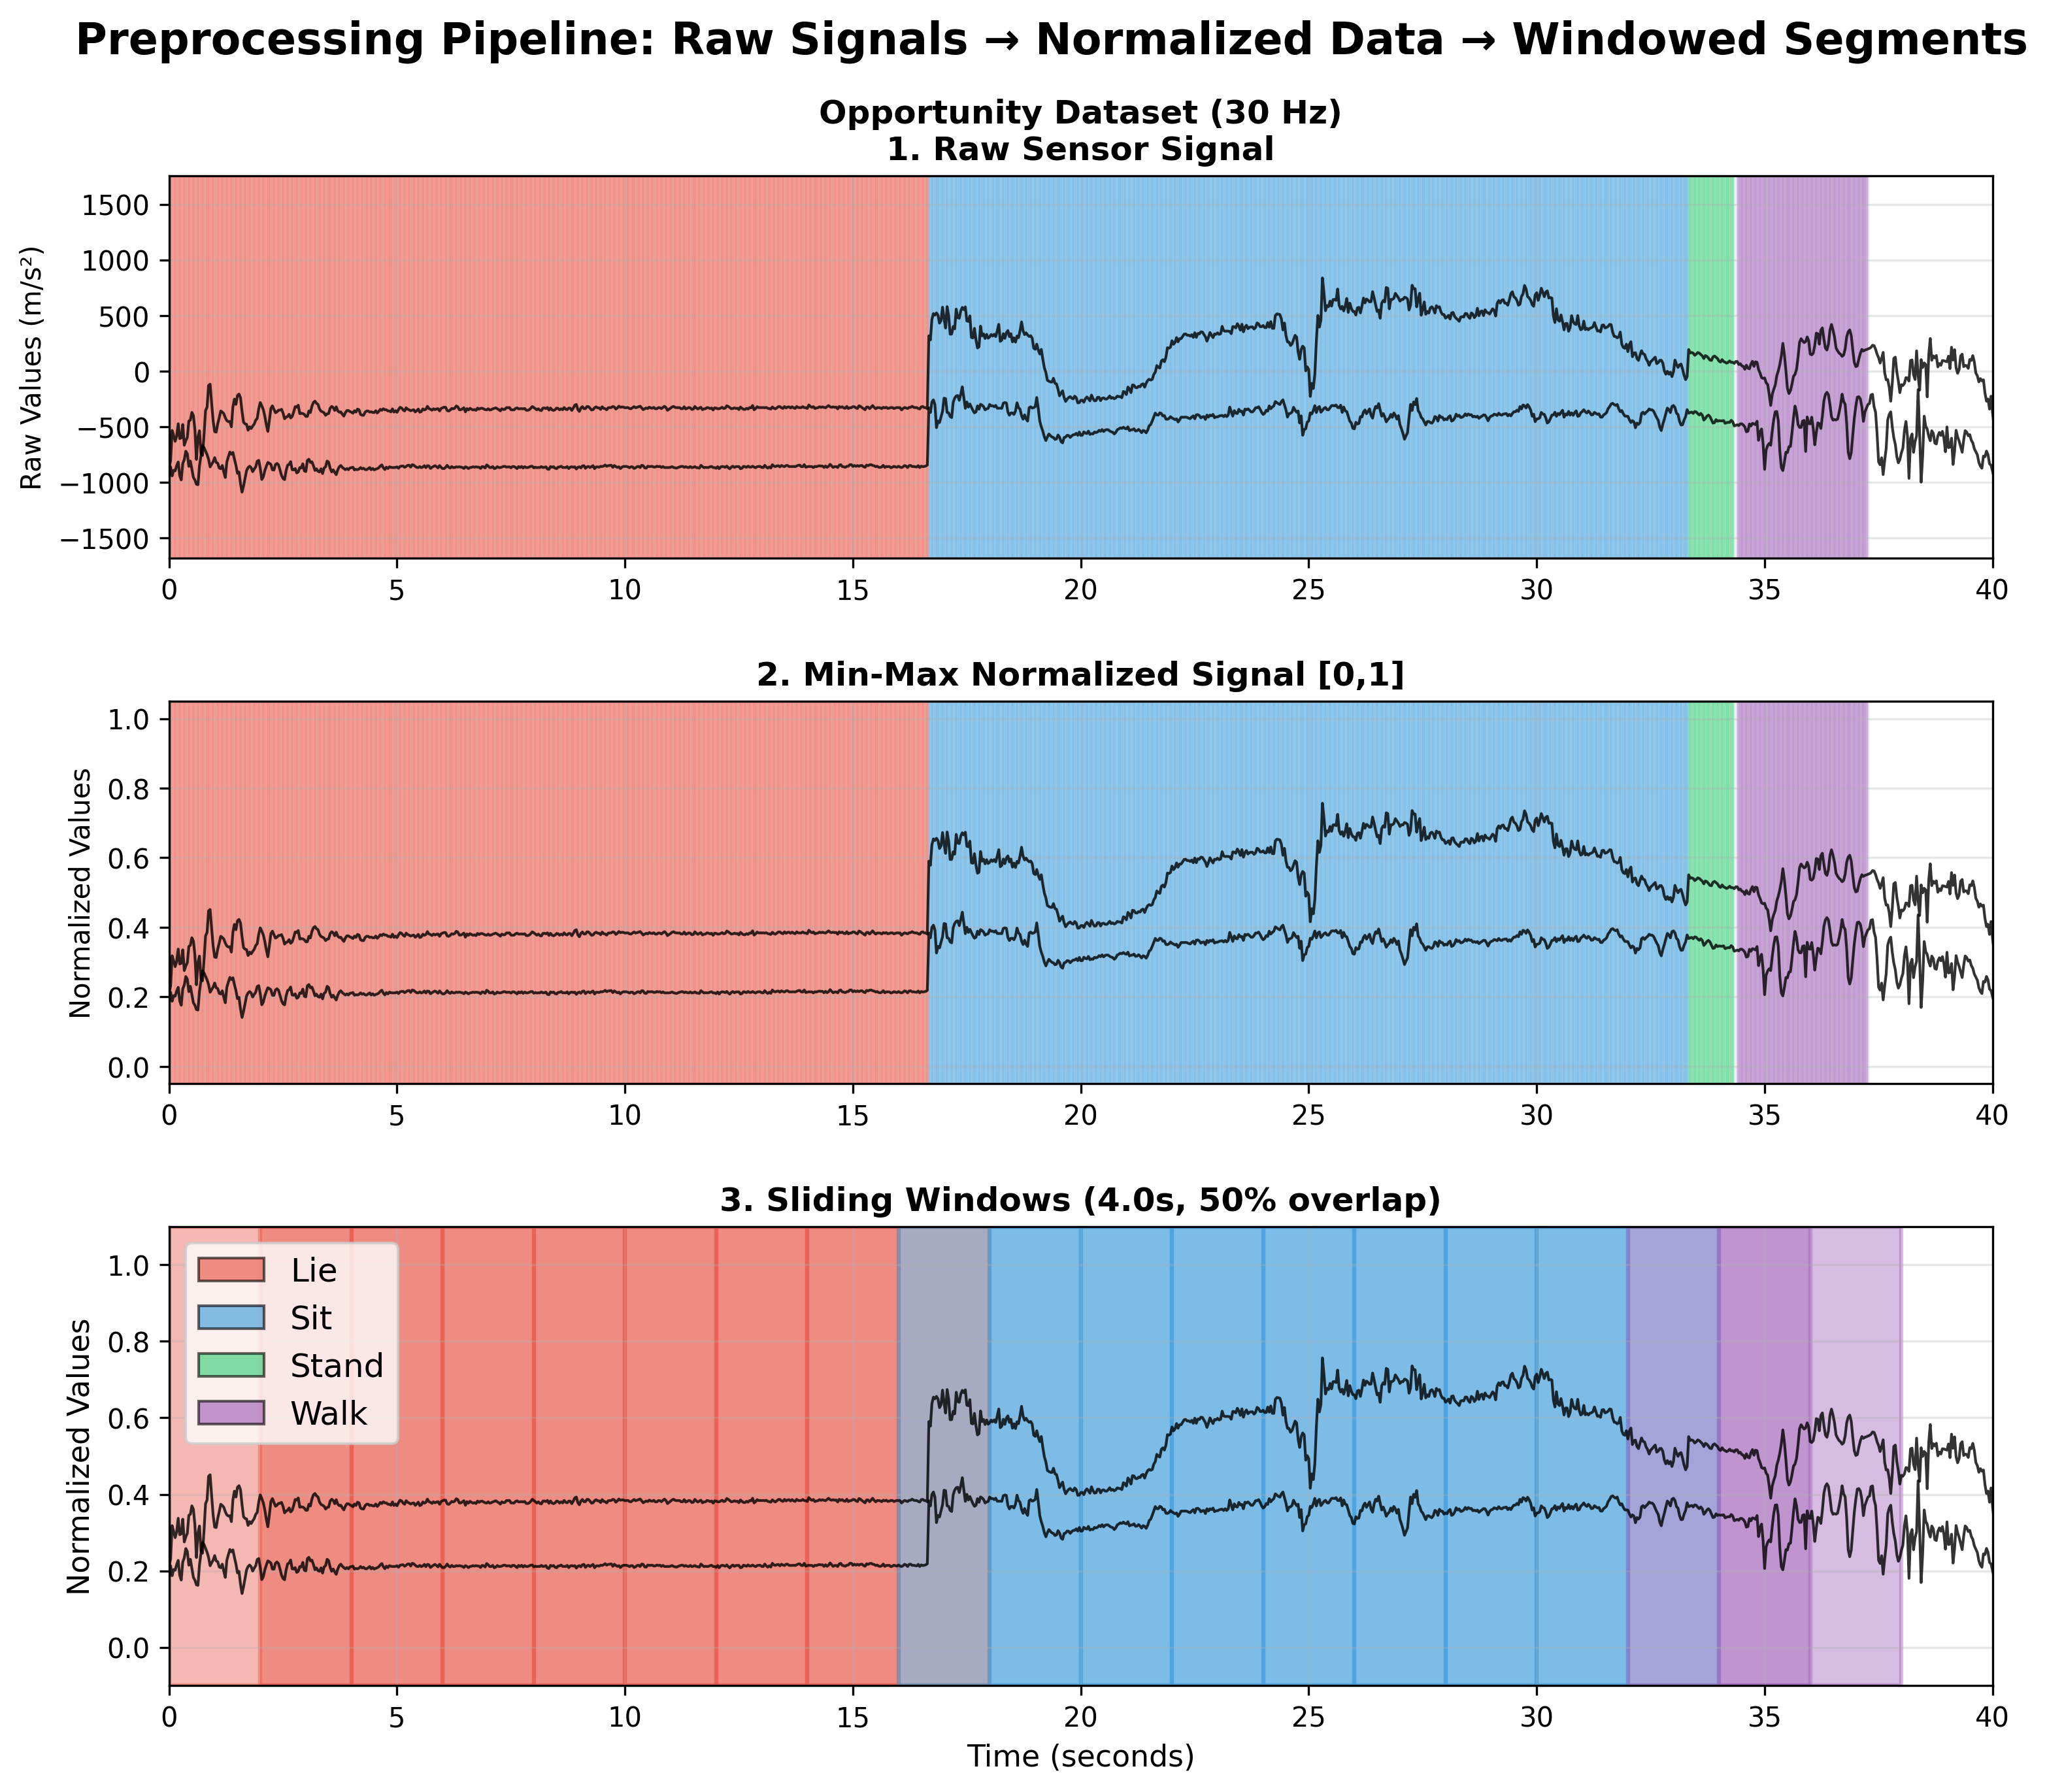
\includegraphics[width=0.9\textwidth]{images/chapter4_preprocessing_pipeline_opportunity.png}
    \caption{Διαδικασία προεπεξεργασίας χρονοσειρών αισθητήρων. Απεικονίζεται η πλήρης αλυσίδα από τα ακατέργαστα σήματα του συνόλου \en{OPPORTUNITY} μέσω κανονικοποίησης \en{min-max} στην επικαλυπτόμενη παραθυροποίηση με απόδοση ετικετών βάσει πλειοψηφικού κανόνα.}
    \label{fig:preprocessing_pipeline}
\end{figure}

\section{Παραγωγή Ασαφών Συναρτήσεων Συμμετοχής}

Η μετάβαση από τα κανονικοποιημένα παράθυρα στις ασαφείς αναπαραστάσεις αποτελεί το κεντρικό βήμα της μεθοδολογίας.
Η παρούσα εργασία συγκρίνει τρεις προσεγγίσεις:

\subsection{\en{Kernel Density Estimation (KDE)}}
Η \en{state of the art} μέθοδος \en{KDE} εκτιμά τη συνάρτηση πυκνότητας $f(x)$ ως:
\[
f(x) = \frac{1}{nh} \sum_{i=1}^{n} K\left(\frac{x - x_i}{h}\right)
\]
όπου $K$ είναι ο πυρήνας (συνήθως \en{Gaussian}), $h$ το εύρος ζώνης (\en{bandwidth}), και $n$ το πλήθος των σημείων. Παρά την υψηλή ακρίβεια, η \en{KDE} απαιτεί σημαντικούς πόρους μνήμης για την αποθήκευση όλων των δεδομένων εκπαίδευσης.

\subsection{\en{Normal Distribution Generator (NDG)}}
Ο αλγόριθμος \en{NDG} εκτιμά τη συνάρτηση πυκνότητας χρησιμοποιώντας άθροισμα πυρήνων. Η γενική μορφή είναι:

\[
\mu(x) = \frac{1}{n} \sum_{i=1}^{n} K(x, x_i, \sigma)
\]

όπου $x_i$ τα σημεία δεδομένων, $n$ το πλήθος των δειγμάτων, $\sigma$ η παράμετρος εύρους ζώνης και $K$ ο πυρήνας.

Η υλοποίηση υποστηρίζει διάφορους τύπους πυρήνων:
\begin{itemize}
    \item \textbf{\en{Gaussian}:} Ο πιο συνηθισμένος πυρήνας με ομαλή μείωση
    \item \textbf{\en{Epanechnikov}:} Βέλτιστος πυρήνας ως προς το μέσο τετραγωνικό σφάλμα
    \item \textbf{\en{Triangular}:} Γραμμική μείωση της επιρροής με την απόσταση
    \item \textbf{\en{Uniform}:} Ορθογωνικός πυρήνας με σταθερή τιμή εντός παραθύρου
    \item \textbf{\en{Quartic}:} Πυρήνας με πιο ομαλή μείωση από τον \en{Epanechnikov}
\end{itemize}

Μετά από πειράματα τα οποία θα αναλυθούν εκτενώς στο επόμενο κεφάλαιο, επιλέχθηκε να χρησιμοποιηθεί ο \en{Gaussian} πυρήνας με $\sigma = 0.1$. Οι επιλογές αυτές παρέχουν την καλύτερη ισορροπία μεταξύ ακρίβειας και υπολογιστικής αποδοτικότητας για τα δεδομένα αισθητήρων.

\subsection{\en{Streaming NDG (NDG-S)}}
Ο αλγόριθμος \en{NDG-S} προσαρμόζει τον \en{NDG} για επεξεργασία μεγάλων δεδομένων μέσω τμηματικής (\en{chunked}) επεξεργασίας:

\begin{enumerate}
    \item \textbf{Τμηματοποίηση δεδομένων:} Τα δεδομένα διαιρούνται σε τμήματα (\en{chunks}), με μέγεθος προσαρμόσιμο ανάλογα με τη διαθέσιμη μνήμη.
    
    \item \textbf{Επεξεργασία ανά τμήμα:} Για κάθε τμήμα $C_k$ υπολογίζεται μερική συνάρτηση συμμετοχής:
    \[
    \mu_k(x) = \frac{1}{|C_k| \sigma \sqrt{2\pi}} \sum_{x_i \in C_k} \exp\left(-\frac{(x - x_i)^2}{2\sigma^2}\right)
    \]
    
    \item \textbf{Συνδυασμός αποτελεσμάτων:} Η τελική συνάρτηση συμμετοχής προκύπτει από το μέσο όρο των μερικών συναρτήσεων:
    \[
    \mu(x) = \frac{1}{K} \sum_{k=1}^{K} \mu_k(x)
    \]
    όπου $K$ ο αριθμός των τμημάτων.
\end{enumerate}

Η διαφορά με τον κλασικό \en{NDG} είναι ότι ο \en{NDG-S} μπορεί να επεξεργαστεί δεδομένα που δεν χωρούν στη μνήμη, με το κόστος ελαφρώς μειωμένης ακρίβειας λόγω της τμηματικής επεξεργασίας.

\subsection{Προσέγγιση Ανά Αισθητήρα}

Στη μετάβαση από τον χρονικό χώρο των δεδομένων αισθητήρων στον χώρο των ασαφών συναρτήσεων συμμετοχής, υπήρχαν πολλές επιλογές για το πώς να συνδυάσουμε τα δεδομένα των διαφορετικών αισθητήρων.
Η επιλογή του υπολογισμού μιας συνάρτησης συμμετοχής ανά αισθητήρα έγινε συνειδητά για να εξυπηρετήσει τον διπλό στόχο της έρευνας: όχι μόνο την αναγνώριση δραστηριοτήτων αλλά και την αναγνώριση του τύπου και της θέσης των αισθητήρων.

Η προσέγγιση αυτή παράγει μία ξεχωριστή συνάρτηση συμμετοχής για κάθε αισθητήρα, διατηρώντας έτσι τα μοναδικά χαρακτηριστικά και την πληροφορία που φέρει ο καθένας. Αυτό επιτρέπει την ταυτόχρονη ανάλυση τόσο του περιεχομένου (τι δραστηριότητα εκτελείται) όσο και της πηγής (ποιος αισθητήρας την κατέγραψε).

\begin{figure}[ht]
    \centering
    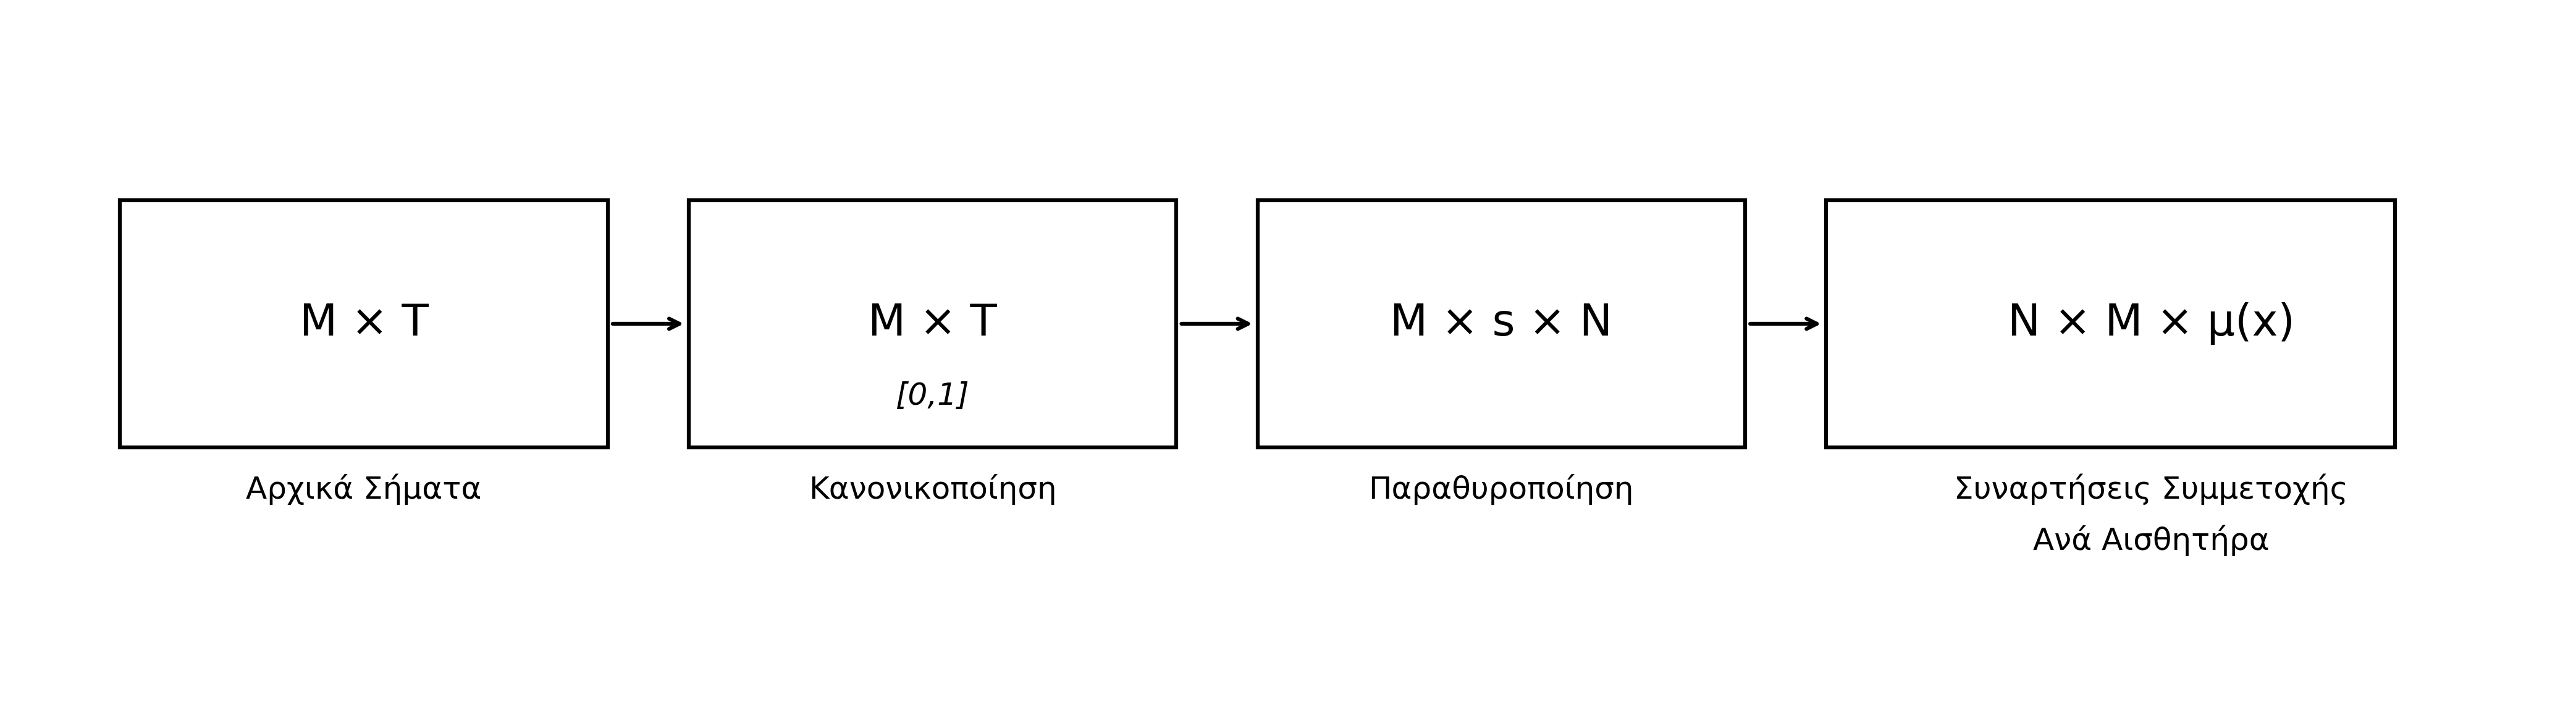
\includegraphics[width=0.9\textwidth]{images/minimal_per_sensor_flow.png}
    \caption{Διαστάσεις δεδομένων στην προσέγγιση ανά αισθητήρα, από τα αρχικά σήματα (\en{M×T}) έως τις τελικές \en{membership functions} (\en{N×M×μ(x)}). Όπου \en{M}: αριθμός αισθητήρων, \en{T}: χρονικά δείγματα, \en{s}: μέγεθος παραθύρου, \en{N}: αριθμός παραθύρων, \en{μ(x)}: \en{membership function values}}
    \label{fig:per_sensor_flow}
\end{figure}

\section{Πλαίσιο Μετρικών Ομοιότητας}

Η σύγκριση των ασαφών συναρτήσεων συμμετοχής απαιτεί εξειδικευμένες μετρικές που λαμβάνουν υπόψη τη συνεχή φύση των τιμών συμμετοχής στο διάστημα $[0,1]$. Η παρούσα εργασία υλοποιεί και αξιολογεί 16 μετρικές ομοιότητας που κατηγοριοποιούνται σε πέντε βασικές οικογένειες.

\subsection{Συνολοθεωρητικές Μετρικές}
Βασισμένες στη θεωρία ασαφών συνόλων, οι μετρικές αυτές εκμεταλλεύονται τις έννοιες της τομής και της ένωσης:

\begin{itemize}
    \item \textbf{\en{Jaccard Similarity}}: $J(\mu_1, \mu_2) = \frac{\int \min(\mu_1(x), \mu_2(x)) dx}{\int \max(\mu_1(x), \mu_2(x)) dx}$
    \item \textbf{\en{Dice Coefficient}}: $D(\mu_1, \mu_2) = \frac{2 \int \min(\mu_1(x), \mu_2(x)) dx}{\int \mu_1(x) dx + \int \mu_2(x) dx}$
    \item \textbf{\en{Overlap Coefficient}}: $O(\mu_1, \mu_2) = \frac{\int \min(\mu_1(x), \mu_2(x)) dx}{\min(\int \mu_1(x) dx, \int \mu_2(x) dx)}$
\end{itemize}

\subsection{Μετρικές Βασισμένες σε Απόσταση}
Μετατρέπουν μετρικές απόστασης σε μέτρα ομοιότητας:

\begin{itemize}
    \item \textbf{\en{Euclidean Similarity}}: $s_E = \frac{1}{1 + \sqrt{\sum_i (\mu_1(x_i) - \mu_2(x_i))^2}}$
    \item \textbf{\en{Hamming Similarity}}: Βασισμένη σε $s_H = \frac{1}{1 + \sum_i |\mu_1(x_i) - \mu_2(x_i)|}$
    \item \textbf{\en{Chebyshev Similarity}}: $s_C = 1 - \max_i |\mu_1(x_i) - \mu_2(x_i)|$ (για $[0,1]$ τιμές)
\end{itemize}

\subsection{Μετρικές Συσχέτισης}
Μετρούν γραμμικές και μη-γραμμικές σχέσεις μεταξύ των συναρτήσεων συμμετοχής:

\begin{itemize}
    \item \textbf{\en{Cosine Similarity}}: $\cos(\mu_1, \mu_2) = \frac{\sum_i \mu_1(x_i) \mu_2(x_i)}{\sqrt{\sum_i \mu_1^2(x_i)} \sqrt{\sum_i \mu_2^2(x_i)}}$
    \item \textbf{\en{Pearson Correlation}}: $r = \frac{\sum_i (\mu_1(x_i) - \bar{\mu_1})(\mu_2(x_i) - \bar{\mu_2})}{\sqrt{\sum_i (\mu_1(x_i) - \bar{\mu_1})^2} \sqrt{\sum_i (\mu_2(x_i) - \bar{\mu_2})^2}}$
    \item \textbf{\en{Cross-Correlation}}: Μέγιστη συσχέτιση με χρονικές μετατοπίσεις
\end{itemize}

\subsection{Πληροφοριοθεωρητικές Μετρικές}
Βασισμένες σε έννοιες από τη θεωρία πληροφοριών και την εντροπία:

\begin{itemize}
    \item \textbf{\en{Jensen-Shannon Similarity}}: $s_{JS} = 1 - \sqrt{JS(P||Q)}$, όπου $JS = \frac{1}{2}KL(P||M) + \frac{1}{2}KL(Q||M)$
    \item \textbf{\en{Bhattacharyya Coefficient}}: $BC = \sum_i \sqrt{p_i q_i}$
    \item \textbf{\en{Hellinger Similarity}}: $s_H = 1 - \frac{1}{\sqrt{2}}\sqrt{\sum_i (\sqrt{p_i} - \sqrt{q_i})^2}$
    \item \textbf{\en{Mutual Information}}: Βασισμένη σε εκτίμηση \en{histogram}
\end{itemize}

\subsection{Προχωρημένες Μετρικές}
Εξειδικευμένες μετρικές για συγκεκριμένες εφαρμογές:

\begin{itemize}
    \item \textbf{\en{Earth Mover's Distance Similarity}}: $s_{EMD} = \frac{1}{1 + EMD(\mu_1, \mu_2)}$ (βέλτιστη μεταφορά)
    \item \textbf{\en{Energy Distance Similarity}}: $s_E = \frac{1}{1 + |E_{12} - E_{11} - E_{22}|}$ 
    \item \textbf{\en{Harmonic Mean Similarity}}: $s_{HM} = \frac{1}{n}\sum_i \frac{2\mu_1(x_i)\mu_2(x_i)}{\mu_1(x_i) + \mu_2(x_i)}$
\end{itemize}

\subsection{Υπολογιστική Υλοποίηση}
Όλες οι μετρικές υλοποιούνται με διανυσματικές λειτουργίες \en{NumPy} για βέλτιστη απόδοση. Η αριθμητική ολοκλήρωση πραγματοποιείται με τον κανόνα του τραπεζίου, ενώ εφαρμόζεται κανονικοποίηση στο $[0,1]$ όπου απαιτείται.


\section{Πειραματικός Σχεδιασμός}
Η αξιολόγηση ακολουθεί προσέγγιση βασισμένη σε ανάκτηση όπου παράθυρα ερωτημάτων συγκρίνονται με βιβλιοθήκη επισημασμένων παραθύρων χρησιμοποιώντας μετρικές \en{Hit@k} και \en{Mean Reciprocal Rank (MRR)}.

\section{Πρωτόκολλο Αξιολόγησης RQ1}
Οι αλγόριθμοι \en{NDG-S} και \en{KDE} συγκρίνονται σε συνθετικά, \en{Opportunity}, και \en{PAMAP2} σύνολα δεδομένων μετρώντας υπολογιστικό χρόνο, χρήση μνήμης, και ακρίβεια προσέγγισης χρησιμοποιώντας \en{KL-divergence}.

\section{Πρωτόκολλο Αξιολόγησης RQ2}
Όλες οι μετρικές ομοιότητας αξιολογούνται σε εργασίες αναγνώρισης δραστηριοτήτων χρησιμοποιώντας ισορροπημένα σύνολα δεδομένων με στρωματοποιημένη δειγματοληψία, μετρώντας ακρίβεια ανάκτησης για διαφορετικούς τύπους ετικετών (\en{Locomotion}, \en{ML\_Both\_Arms}, \en{HL\_Activity}).

\section{Πρωτόκολλο Αξιολόγησης RQ3}
Η ευστάθεια μεταξύ συνόλων δεδομένων εκτιμάται υπολογίζοντας συσχετίσεις \en{Spearman rank} μεταξύ κατατάξεων απόδοσης μετρικών στα σύνολα δεδομένων \en{Opportunity} και \en{PAMAP2}.

\section{Πλαίσιο Στατιστικής Ανάλυσης}
Η στατιστική σημαντικότητα καθορίζεται χρησιμοποιώντας τεστ \en{Wilcoxon signed-rank} για ζευγαρωτές συγκρίσεις και τεστ \en{Friedman} για συγκρίσεις πολλαπλών μετρικών, με ανάλυση \en{Nemenyi post-hoc} για διαφορές ομάδων.

\section{Βελτιστοποίηση Απόδοσης}
Η ενοποιημένη προσέγγιση παραθύρων προυπολογίζει συναρτήσεις συμμετοχής μία φορά και τις επαναχρησιμοποιεί σε πολλαπλούς τύπους ετικετών, επιτυγχάνοντας σημαντική υπολογιστική επιτάχυνση για πειράματα πολλαπλών ετικετών.

\section{Στρατηγική Επικύρωσης}
Η διασταυρούμενη επικύρωση εκτελείται χρησιμοποιώντας στρωματοποιημένες διαιρέσεις για εξασφάλιση ισορροπημένης αναπαράστασης δραστηριοτήτων και τύπων αισθητήρων, με ξεχωριστές κατανομές εκπαίδευσης/ελέγχου για αποφυγή διαρροής δεδομένων.

\section{Λεπτομέρειες Υλοποίησης}
Όλοι οι αλγόριθμοι υλοποιούνται σε \en{Python} χρησιμοποιώντας \en{NumPy} για διανυσματικές λειτουργίες, με μηχανισμούς προσωρινής αποθήκευσης για συναρτήσεις συμμετοχής και παράλληλη επεξεργασία για υπολογισμούς ομοιότητας.

\section{Μετρικές Αξιολόγησης}
Οι κύριες μετρικές περιλαμβάνουν \en{Hit@1}, \en{Hit@5}, \en{MRR} για εργασίες ανάκτησης, συν μέτρα υπολογιστικής αποδοτικότητας (χρόνος εκτέλεσης, χρήση μνήμης) και δείκτες στατιστικής σημαντικότητας (τιμές \en{p}, μεγέθη επίδρασης).


\section{Σύνοψη κεφαλαίου}
% TODO: Ανακεφαλαίωση και σύνδεση με επόμενο κεφάλαιο.
